% Digital Logic Report Template
% Created: 2020-01-10, John Miller

%==========================================================
%=========== Document Setup  ==============================

% Formatting defined by class file
\documentclass[11pt]{article}

% ---- Document formatting ----
\usepackage[margin=1in]{geometry}	% Narrower margins
\usepackage{booktabs}				% Nice formatting of tables
\usepackage{graphicx}				% Ability to include graphics

%\setlength\parindent{0pt}	% Do not indent first line of paragraphs 
\usepackage[parfill]{parskip}		% Line space b/w paragraphs
%	parfill option prevents last line of pgrph from being fully justified

% Parskip package adds too much space around titles, fix with this
\RequirePackage{titlesec}
\titlespacing\section{0pt}{8pt plus 4pt minus 2pt}{3pt plus 2pt minus 2pt}
\titlespacing\subsection{0pt}{4pt plus 4pt minus 2pt}{-2pt plus 2pt minus 2pt}
\titlespacing\subsubsection{0pt}{2pt plus 4pt minus 2pt}{-6pt plus 2pt minus 2pt}

% ---- Hyperlinks ----
\usepackage[colorlinks=true,urlcolor=blue]{hyperref}	% For URL's. Automatically links internal references.

% ---- Code listings ----
\usepackage{listings} 					% Nice code layout and inclusion
\usepackage[usenames,dvipsnames]{xcolor}	% Colors (needs to be defined before using colors)

% Define custom colors for listings
\definecolor{listinggray}{gray}{0.98}		% Listings background color
\definecolor{rulegray}{gray}{0.7}			% Listings rule/frame color

% Style for Verilog
\lstdefinestyle{Verilog}{
	language=Verilog,					% Verilog
	backgroundcolor=\color{listinggray},	% light gray background
	rulecolor=\color{blue}, 			% blue frame lines
	frame=tb,							% lines above & below
	linewidth=\columnwidth, 			% set line width
	basicstyle=\small\ttfamily,	% basic font style that is used for the code	
	breaklines=true, 					% allow breaking across columns/pages
	tabsize=3,							% set tab size
	commentstyle=\color{gray},	% comments in italic 
	stringstyle=\upshape,				% strings are printed in normal font
	showspaces=false,					% don't underscore spaces
}

% How to use: \Verilog[listing_options]{file}
\newcommand{\Verilog}[2][]{%
	\lstinputlisting[style=Verilog,#1]{#2}
}




%======================================================
%=========== Body  ====================================
\begin{document}

\title{ELC 2137 Lab 1: Introduction to Git and LaTex}
\author{Sam Jeffrey}

\maketitle


\section*{Summary}

In this lab I worked with two diffrent softwares Git and LaTex. Git stores code online so that it can be easily accessible from any device. This allows for others to easily modify and view code. Git also keeps track of modifications to the code, this allows for easy debugging. LaTex creates documents using a typesetting language. This allows for many advantages. The documents are professional grade and can allow for many short cuts when creating documents. Through this lab I familurized myself with these softwares. In Git I synchronized local and online files into a respoitory. Which means I basicaly downloaded and uploaded code to Git. In LaTex I created this document. In creating this document I had to use varius features such as cropping, inserting code and inserting equations. This lab allowed me to start understand these softwares and for me to become faster at using them. 

\section*{Q\&A}


\begin{enumerate}
\item  What is your GitHub user name?
 
Awnser: My user name is samjeffrey1

\item  What  LaTeX  environment  produces  a  bulleted(non-numbered) list?

Awnser: The itemize environment produces bulleted lists.

\item  Write  the  equationy(t) = 1/2 $e^t$ using  La-TeX equation formatting.

Awnser: 
\begin{equation}
	y(t) = \frac{1}{2}e^t
\end{equation}

\item  What is the shortcut key for compiling your La-TeX document?

Awnser: F6 compiles the program

\end{enumerate}


\section*{Results}

For the results section I created figure 1. Inorder to create the table part of figure 1 I created a tabular. In the tabular I was able to input the data and headers. I then ended the tabular and included the picture graphic. When I included the picture graphic I cropped each side using trim feature. This allowed me to create figure 1 which is seen below.

\begin{figure}[ht]\centering
	\begin{tabular}{c|c|c}
		\toprule
		Binary & Hex & Decimal \\
		\midrule
		0000 & 0 & 0 \\
		0010 & 2 & 2 \\
		0100 & 4 & 4 \\
		0110 & 6 & 6 \\
		1000 & 8 & 8 \\
		1010 & A & 10 \\
		\bottomrule
	\end{tabular} 
	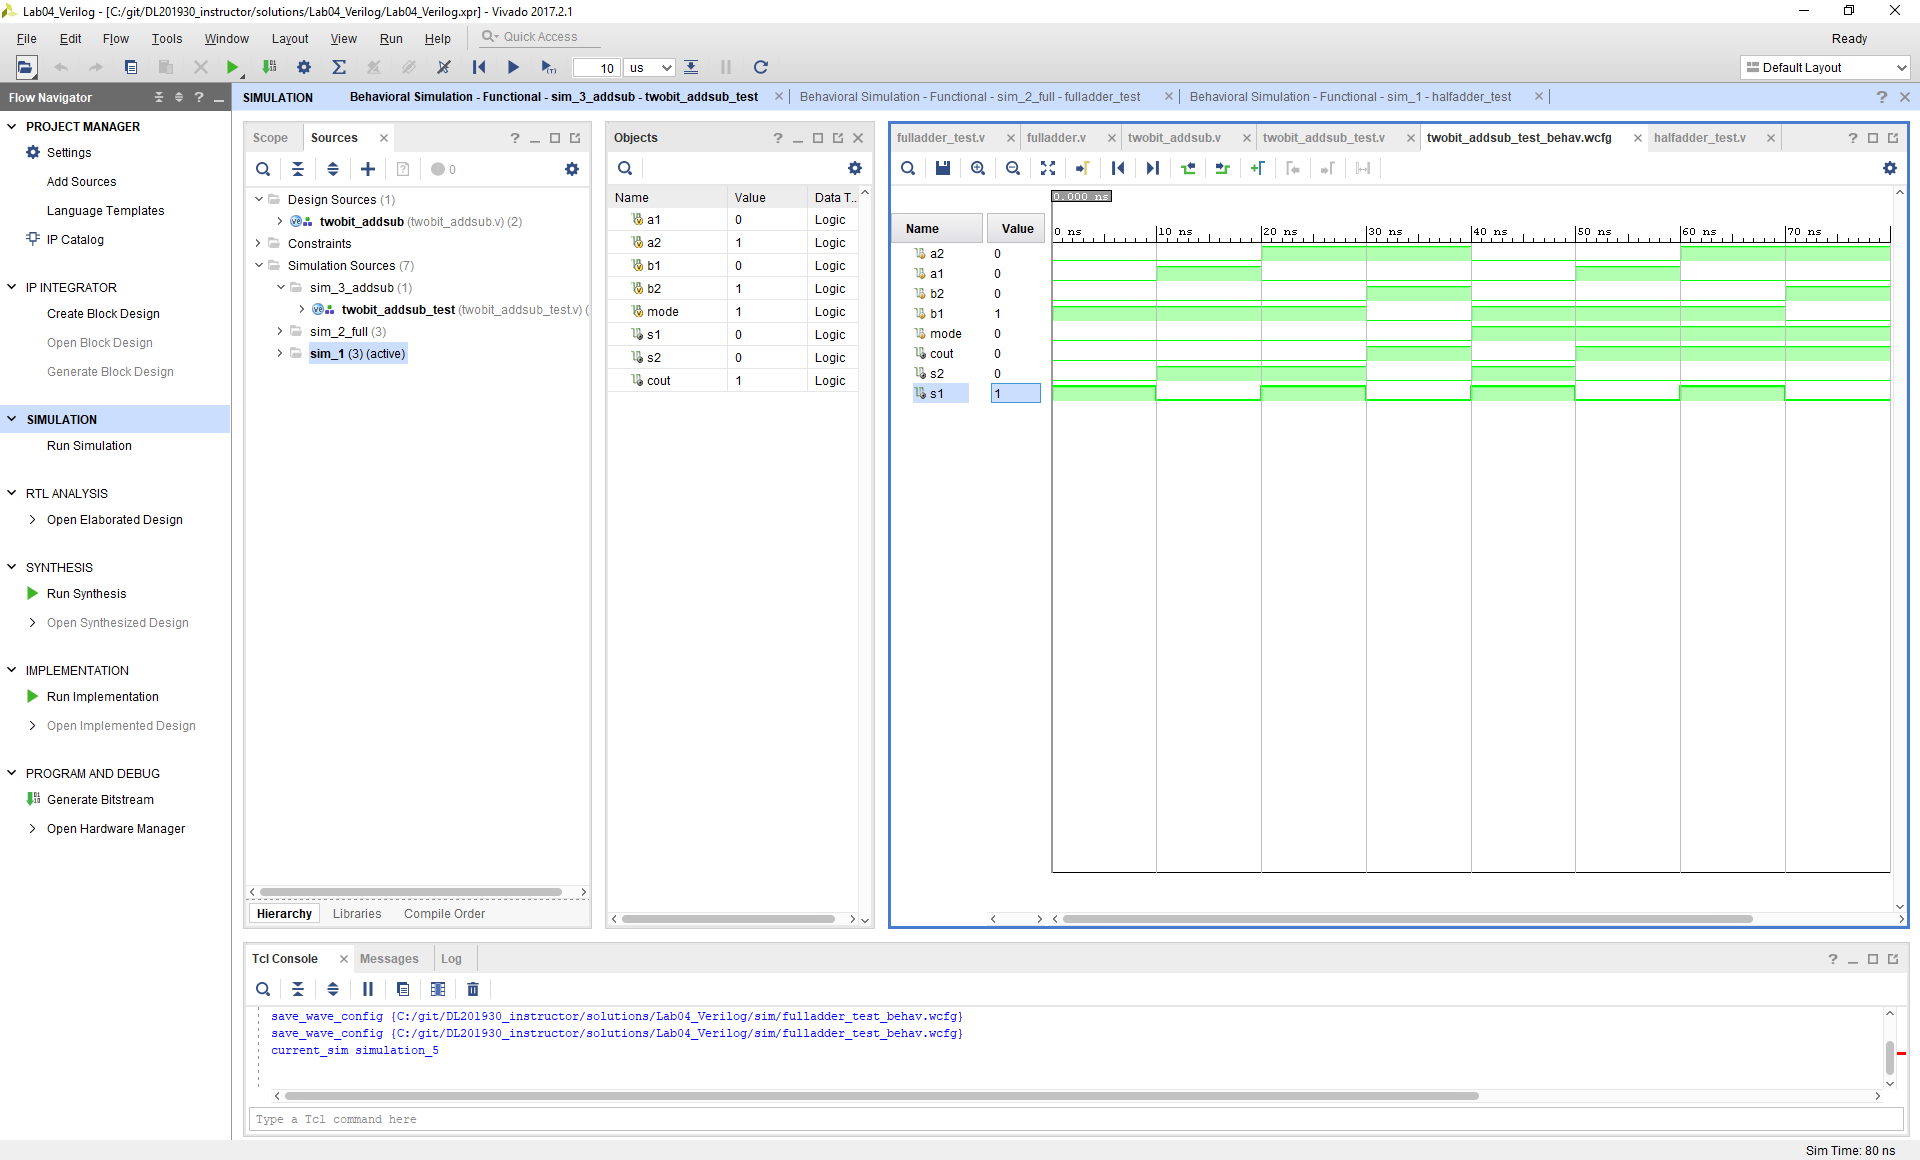
\includegraphics[width=1\textwidth,trim=18.5cm 15.75cm .5cm 4.5cm,clip]{lab1_example_screenshot.PNG}
	\caption{Table and simulation waveform to reproduce}
	\label{fig:another_image}          % label must be after caption
\end{figure}


\section*{Code}

\Verilog[caption=File-included from canvas]{lab1_example_code.sv}


\end{document}
